\section{CReactor  Class Reference}
\label{classCReactor}\index{CReactor@{CReactor}}
{\tt \#include $<$CReactor.h$>$}

Inheritance diagram for CReactor::\begin{figure}[H]
\begin{center}
\leavevmode
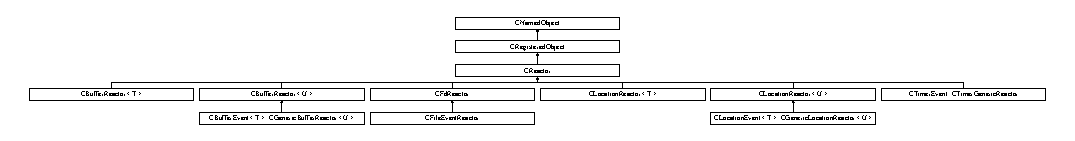
\includegraphics[height=1.44033cm]{classCReactor}
\end{center}
\end{figure}
\subsection*{Public Methods}
\begin{CompactItemize}
\item 
{\bf CReactor} ()
\item 
{\bf CReactor} (const string \&r\-Name)
\item 
{\bf CReactor} (const char $\ast$p\-Name)
\item 
virtual {\bf $\sim$CReactor} ()
\item 
int {\bf operator==} (const CReactor \&a\-CReactor) const
\item 
virtual void {\bf operator()} ({\bf CEvent\-Monitor} \&r\-Monitor, {\bf CEvent\-Monitor::result} Reason)
\item 
virtual void {\bf On\-Event} ({\bf CEvent\-Monitor} \&r\-Monitor)
\item 
virtual void {\bf On\-Error} ({\bf CEvent\-Monitor} \&r\-Monitor)
\item 
virtual void {\bf On\-Timeout} ({\bf CEvent\-Monitor} \&r\-Monitor)
\end{CompactItemize}
\subsection*{Private Methods}
\begin{CompactItemize}
\item 
{\bf CReactor} (const CReactor \&a\-CReactor)
\begin{CompactList}\small\item\em For now copy construction is not allowed.\item\end{CompactList}\item 
CReactor \& {\bf operator=} (const CReactor \&a\-CReactor)
\begin{CompactList}\small\item\em For now assignment is illegal.\item\end{CompactList}\end{CompactItemize}


\subsection{Detailed Description}
Encapsulates the base class for reactors. A reactor is an object which responds to an  event. This class hierarchy is of necessity slightly parallel to the Monitor hierarchy. In additional to the Named Object standard functions, all monitors must implement:\begin{CompactItemize}
\item 
operator() - called when the monitor fires.\end{CompactItemize}
\begin{CompactItemize}
\item 
{\bf On\-Event}() {\rm (p.\,\pageref{classCReactor_a6})} - Called from operator() if an event fired.\item 
{\bf On\-Error}() {\rm (p.\,\pageref{classCReactor_a7})} - Called from operator() if a monitor detected and error.\item 
{\bf On\-Timeout}() {\rm (p.\,\pageref{classCReactor_a8})}- Called from operator() if a monitor deteted a timeout.\end{CompactItemize}
As a named object, CReactor's require a name on construction. The name is entered into the \char`\"{}Reactor\char`\"{} registry. As a convenience, a default  constructor is supplied, however. If used the default constructor generates a name of the form Reactor\_\-nnn where nnn is a unique number... from m\_\-Auto\-Index.

This base class provides: Get\-Auto\-Name member function for derived classes which desire to implement this functionality as well. 



Definition at line 331 of file CReactor.h.

\subsection{Constructor \& Destructor Documentation}
\index{CReactor@{CReactor}!CReactor@{CReactor}}
\index{CReactor@{CReactor}!CReactor@{CReactor}}
\subsubsection{\setlength{\rightskip}{0pt plus 5cm}CReactor::CReactor ()}\label{classCReactor_a0}


Default constructor. A Reactor with name of the form Reactor\_\-nnn is created. The reactor is entered in to the \char`\"{}Reactor\char`\"{} registry of the  classified object registry returned from get\-CClassified\-Object\-Registry(). The name used is gaurenteed unique and can be queried via: {\bf get\-Name}() {\rm (p.\,\pageref{classCNamedObject_a6})}. 

Definition at line 321 of file CReactor.cpp.

References CNamed\-Object::Append\-Class\-Info(), and Registry\-Name.\index{CReactor@{CReactor}!CReactor@{CReactor}}
\index{CReactor@{CReactor}!CReactor@{CReactor}}
\subsubsection{\setlength{\rightskip}{0pt plus 5cm}CReactor::CReactor (const string \& {\em r\-Name})}\label{classCReactor_a1}


Constructs a Reactor given a name as an STL string:\begin{Desc}
\item[Parameters: ]\par
\begin{description}
\item[{\em 
r\-Name}]- The desired name of the reactor.\end{description}
\end{Desc}
Throws:\begin{CompactItemize}
\item 
{\bf CDuplicate\-Name\-Exception} {\rm (p.\,\pageref{classCDuplicateNameException})} (indirectly) if a Reactor of this name already exists. \end{CompactItemize}


Definition at line 337 of file CReactor.cpp.

References CNamed\-Object::Append\-Class\-Info(), and Registry\-Name.\index{CReactor@{CReactor}!CReactor@{CReactor}}
\index{CReactor@{CReactor}!CReactor@{CReactor}}
\subsubsection{\setlength{\rightskip}{0pt plus 5cm}CReactor::CReactor (const char $\ast$ {\em p\-Name})}\label{classCReactor_a2}


Constructs a reactor given its name as an ASCIZ string:\begin{Desc}
\item[Parameters: ]\par
\begin{description}
\item[{\em 
p\-Name}]- char$\ast$ pointer to the desired object name.\end{description}
\end{Desc}
Throws: -{\bf CDuplicate\-Name\-Exception} {\rm (p.\,\pageref{classCDuplicateNameException})} (indirectly) if a Reactor of this name already exists. 

Definition at line 354 of file CReactor.cpp.

References CNamed\-Object::Append\-Class\-Info(), and Registry\-Name.\index{CReactor@{CReactor}!CReactor@{CReactor}}
\index{CReactor@{CReactor}!CReactor@{CReactor}}
\subsubsection{\setlength{\rightskip}{0pt plus 5cm}CReactor::CReactor (const CReactor \& {\em a\-CReactor})\hspace{0.3cm}{\tt  [private]}}\label{classCReactor_c0}


For now copy construction is not allowed.

\index{CReactor@{CReactor}!~CReactor@{$\sim$CReactor}}
\index{~CReactor@{$\sim$CReactor}!CReactor@{CReactor}}
\subsubsection{\setlength{\rightskip}{0pt plus 5cm}CReactor::$\sim$CReactor ()\hspace{0.3cm}{\tt  [virtual]}}\label{classCReactor_a3}


Destructor: Just ensure that we are removed from the Reactors registry before being destroyed. 

Definition at line 366 of file CReactor.cpp.

References CApplication\-Registry::get\-Instance(), Registry\-Name, and CClassified\-Object\-Registry::Remove().

\subsection{Member Function Documentation}
\index{CReactor@{CReactor}!OnError@{OnError}}
\index{OnError@{OnError}!CReactor@{CReactor}}
\subsubsection{\setlength{\rightskip}{0pt plus 5cm}void CReactor::On\-Error ({\bf CEvent\-Monitor} \& {\em r\-Event})\hspace{0.3cm}{\tt  [virtual]}}\label{classCReactor_a7}


Called when the event monitor detects an error while waiting for an event. In general, this class is subclassed, and the actual code for On\-Error is supplied by the subclass. In order to support classes which may not care about event monitor errors themselves,  we provide an empty implementation of this function, preventing us from being an ABC.\begin{Desc}
\item[Parameters: ]\par
\begin{description}
\item[{\em 
r\-Monitor}]- The monitor which detected the event. \end{description}
\end{Desc}


Definition at line 447 of file CReactor.cpp.

Referenced by operator()().\index{CReactor@{CReactor}!OnEvent@{OnEvent}}
\index{OnEvent@{OnEvent}!CReactor@{CReactor}}
\subsubsection{\setlength{\rightskip}{0pt plus 5cm}void CReactor::On\-Event ({\bf CEvent\-Monitor} \& {\em r\-Event})\hspace{0.3cm}{\tt  [virtual]}}\label{classCReactor_a6}


Called when the event occurs. This is called from operator(). In general, this class is subclassed, and the actual code for On\-Event is supplied by the subclass. In order to support classes which may not care about the event themselves, we provide an empty implementation of this function, preventing us from being an ABC.\begin{Desc}
\item[Parameters: ]\par
\begin{description}
\item[{\em 
r\-Monitor}]- The monitor which detected the event. \end{description}
\end{Desc}


Reimplemented in {\bf CBuffer\-Reactor$<$ T $>$} {\rm (p.\,\pageref{classCBufferReactor_a5})}, {\bf CFd\-Reactor} {\rm (p.\,\pageref{classCFdReactor_a5})}, {\bf CLocation\-Reactor$<$ T $>$} {\rm (p.\,\pageref{classCLocationReactor_a5})}, {\bf CTimer\-Event::CTimer\-Generic\-Reactor} {\rm (p.\,\pageref{classCTimerEvent_1_1CTimerGenericReactor_a2})}, {\bf CBuffer\-Reactor$<$ U $>$} {\rm (p.\,\pageref{classCBufferReactor_a5})}, and {\bf CLocation\-Reactor$<$ U $>$} {\rm (p.\,\pageref{classCLocationReactor_a5})}.

Definition at line 433 of file CReactor.cpp.

Referenced by operator()().\index{CReactor@{CReactor}!OnTimeout@{OnTimeout}}
\index{OnTimeout@{OnTimeout}!CReactor@{CReactor}}
\subsubsection{\setlength{\rightskip}{0pt plus 5cm}void CReactor::On\-Timeout ({\bf CEvent\-Monitor} \& {\em r\-Event})\hspace{0.3cm}{\tt  [virtual]}}\label{classCReactor_a8}


Called when an event monitor detects a timeout while waiting for the event. In general, this class is subclassed, and the actual code for On\-Timeout is supplied by the subclass. In order to support classes which may not care about event monitor timeouts themselves,  we provide an empty implementation of this function, preventing us from being an ABC.\begin{Desc}
\item[Parameters: ]\par
\begin{description}
\item[{\em 
r\-Monitor}]- The monitor which detected the event. \end{description}
\end{Desc}


Reimplemented in {\bf CBuffer\-Event$<$ T $>$::CGeneric\-Buffer\-Reactor$<$ U $>$} {\rm (p.\,\pageref{classCBufferEvent_1_1CGenericBufferReactor_a2})}, {\bf CFile\-Event\-Reactor} {\rm (p.\,\pageref{classCFileEvent_1_1CFileEventReactor_a5})}, {\bf CLocation\-Event$<$ T $>$::CGeneric\-Location\-Reactor$<$ U $>$} {\rm (p.\,\pageref{classCLocationEvent_1_1CGenericLocationReactor_a2})}, and {\bf CBuffer\-Event$<$ T $>$::CGeneric\-Buffer\-Reactor$<$ T $>$} {\rm (p.\,\pageref{classCBufferEvent_1_1CGenericBufferReactor_a2})}.

Definition at line 461 of file CReactor.cpp.

Referenced by operator()().\index{CReactor@{CReactor}!operator()@{operator()}}
\index{operator()@{operator()}!CReactor@{CReactor}}
\subsubsection{\setlength{\rightskip}{0pt plus 5cm}void CReactor::operator() ({\bf CEvent\-Monitor} \& {\em r\-Monitor}, {\bf CEvent\-Monitor::result} {\em Reason})\hspace{0.3cm}{\tt  [virtual]}}\label{classCReactor_a5}


Operation Type: Interface Definition

Purpose:

This method is called in response ot an event from an event monitor on which this reactor has been established. The Reactor provides  application specific procesing of the event.\begin{Desc}
\item[Parameters: ]\par
\begin{description}
\item[{\em 
r\-Monitor}]- The event monitor which fired off our reaction. \item[{\em 
Reason}]- Why we were fired. Can be any of:\begin{CompactItemize}
\item 
Ocurred - the event happened.\item 
Timed\-Out - The event did not happen within the timeout.\item 
Error - Some error occured on the event.\end{CompactItemize}
\end{description}
\end{Desc}
Throws:\begin{CompactItemize}
\item 
{\bf CRange\-Error} {\rm (p.\,\pageref{classCRangeError})} if an invalid Reason was passed in. \end{CompactItemize}


Definition at line 404 of file CReactor.cpp.

References CEvent\-Monitor::Error, CEvent\-Monitor::Occurred, On\-Error(), On\-Event(), On\-Timeout(), CEvent\-Monitor::result, and CEvent\-Monitor::Timed\-Out.\index{CReactor@{CReactor}!operator=@{operator=}}
\index{operator=@{operator=}!CReactor@{CReactor}}
\subsubsection{\setlength{\rightskip}{0pt plus 5cm}CReactor\& CReactor::operator= (const CReactor \& {\em a\-CReactor})\hspace{0.3cm}{\tt  [private]}}\label{classCReactor_c1}


For now assignment is illegal.

\index{CReactor@{CReactor}!operator==@{operator==}}
\index{operator==@{operator==}!CReactor@{CReactor}}
\subsubsection{\setlength{\rightskip}{0pt plus 5cm}int CReactor::operator== (const CReactor \& {\em a\-CReactor}) const}\label{classCReactor_a4}




Definition at line 374 of file CReactor.cpp.

References CRegistered\-Object::operator==().

Referenced by CLocation\-Reactor$<$ T $>$::operator==(), CFd\-Reactor::operator==(), and CBuffer\-Reactor$<$ T $>$::operator==().

The documentation for this class was generated from the following files:\begin{CompactItemize}
\item 
{\bf CReactor.h}\item 
{\bf CReactor.cpp}\end{CompactItemize}
